\documentclass[../../main.tex]{subfiles}

 \lhead{Implementation: Room Modelling}
 
\begin{document}
	\subsection{Room Modelling}

		\subsubsection{Room Measurements}

			Before taking room measurements, a quick top-down map of the room was made, highlighting objects, wall indents or protrusions as well as where doors and windows existed. The dimensions of the room were then measured in meters and noted on the not to scale room map. The tool used for taking measurements was a DeWalt laser distance measurer \cite{dewalt}, allowing for accurate measurements of distances that would otherwise not be accessible such as the distance between the lights on the roof. Once the basic layout had been mapped, more detailed diagrams of individual walls were made, paying close attention to window and door dimensions, distances between doors and window panes, the depth of the radiators on the walls etc, as these small variations in surface depth would greatly influence how sound would reflect around the room. An example of an annotated blueprint can be seen in figure~\ref{blueprintTop} in \nameref{appendixA}.

			The dimensions of Hendrix Hall were measured at approximately 18.3m x 18.2m x 5.5m.

		\subsubsection{Designing the room}
			\label{designRoom}
			The blue prints were used to model the room in Google SketchUp starting with a hollow rectangle with the dimensions of Hendrix Hall. The wall indents and protrusions were then modelled by using a push/pull tool. Figure~\ref{sku1} shows an early iteration of the SketchUp model where several wall protrusions have been modelled.

			%-------------Early SketchUp Model Image-------------%
			\begin{figure}[ht]
				\center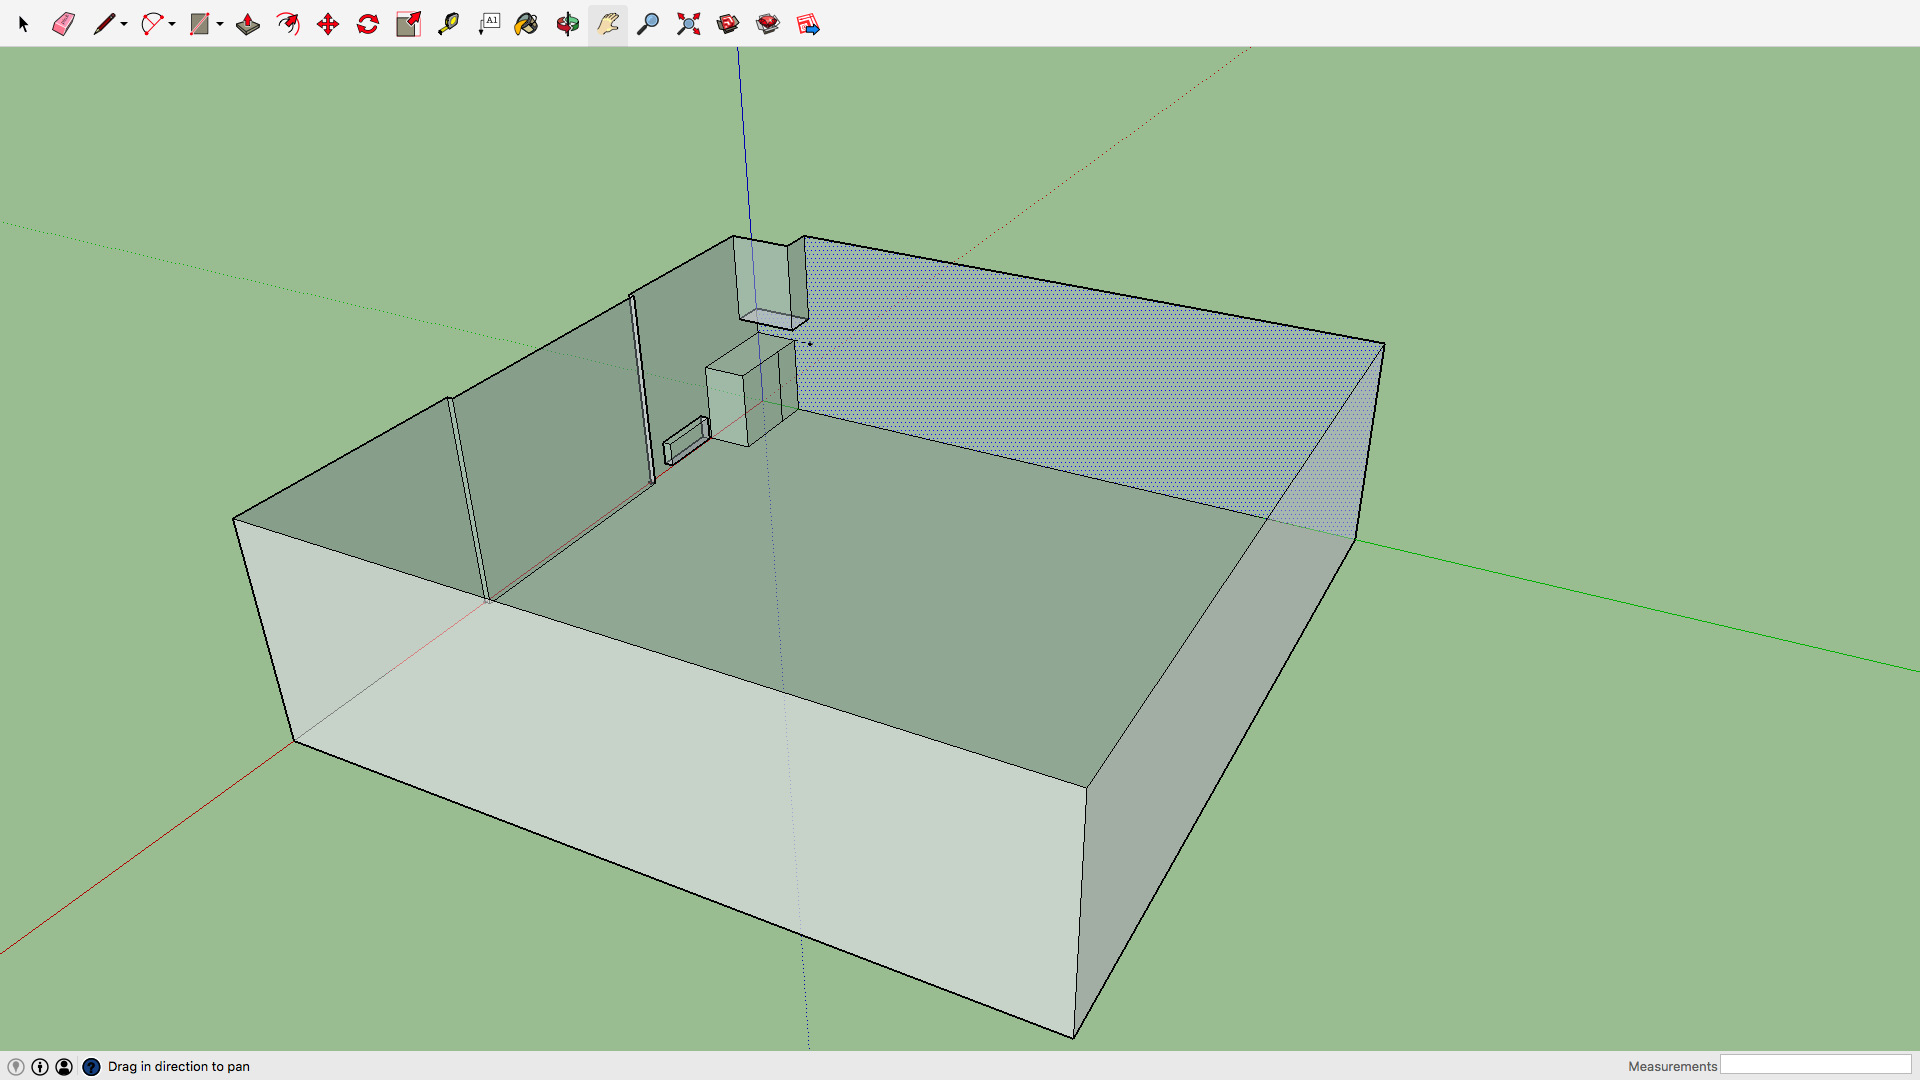
\includegraphics[scale = 0.2]{Sections/Implementation/Modelling/images/sku1.png}
				\caption{Early iteration of the Hendrix Hall SketchUp model with a few early wall protrusions being modelled such as the entrance door, a radiator and one of the wall indents.}
				\label{sku1}
			\end{figure}

			Hendrix Hall predominantly consists of flat surfaces, though some more complex surfaces include:

			\begin{itemize}
				\item[-] Lights (concave curves) 
				\item[-] Canvas roof hangings (convex curves) 
				\item[-] Projector hangings (poles)
				%\item[-] Roof (tiled) 
				\item[-] Radiator, door and vent grills \\
			\end{itemize}

			These objects were initially designed to look as close to the real thing as possible, however the objects with curved edges posed a problem when importing the model into Odeon. This is because SketchUp uses a large number of short surfaces to represent curves, as can be seen on the left of Figure~\ref{compareModels} which shows the initial models of the lights, projectors and roof hangings. According to the Odeon manual \cite{odeonManual}, when modelling a room for acoustic simulation purposes it is more accurate and less time consuming to keep the model simple and to add the appropriate scattering coefficients or materials in Odeon itself. This also applied to the objects (such as the radiators) that contained a grilled surface, as a specific `grill' material could be selected from Odeons material list (see section \nameref{odeon:materials}).

			The objects were redesigned to Odeons specifications by using simple geometry, where the roof hangings were represented as four joint slanting surfaces and the lights and projector poles were represented as simple rectangles, as can be seen on the right in figure~\ref{compareModels}

			Images of the final model compared to the real room can be found in \nameref{appendixA}, in figures \ref{comp1}, \ref{comp2} and \ref{comp3}, showing that the room was carefully recreated in hope of improving the accuracy of the results obtained from Odeon. The Google Sketchup file is also available in folder 4.1 as part of the supporting material.



						%-------------Lights and projector images-------------%
			\begin{figure}[H]
				\centerline{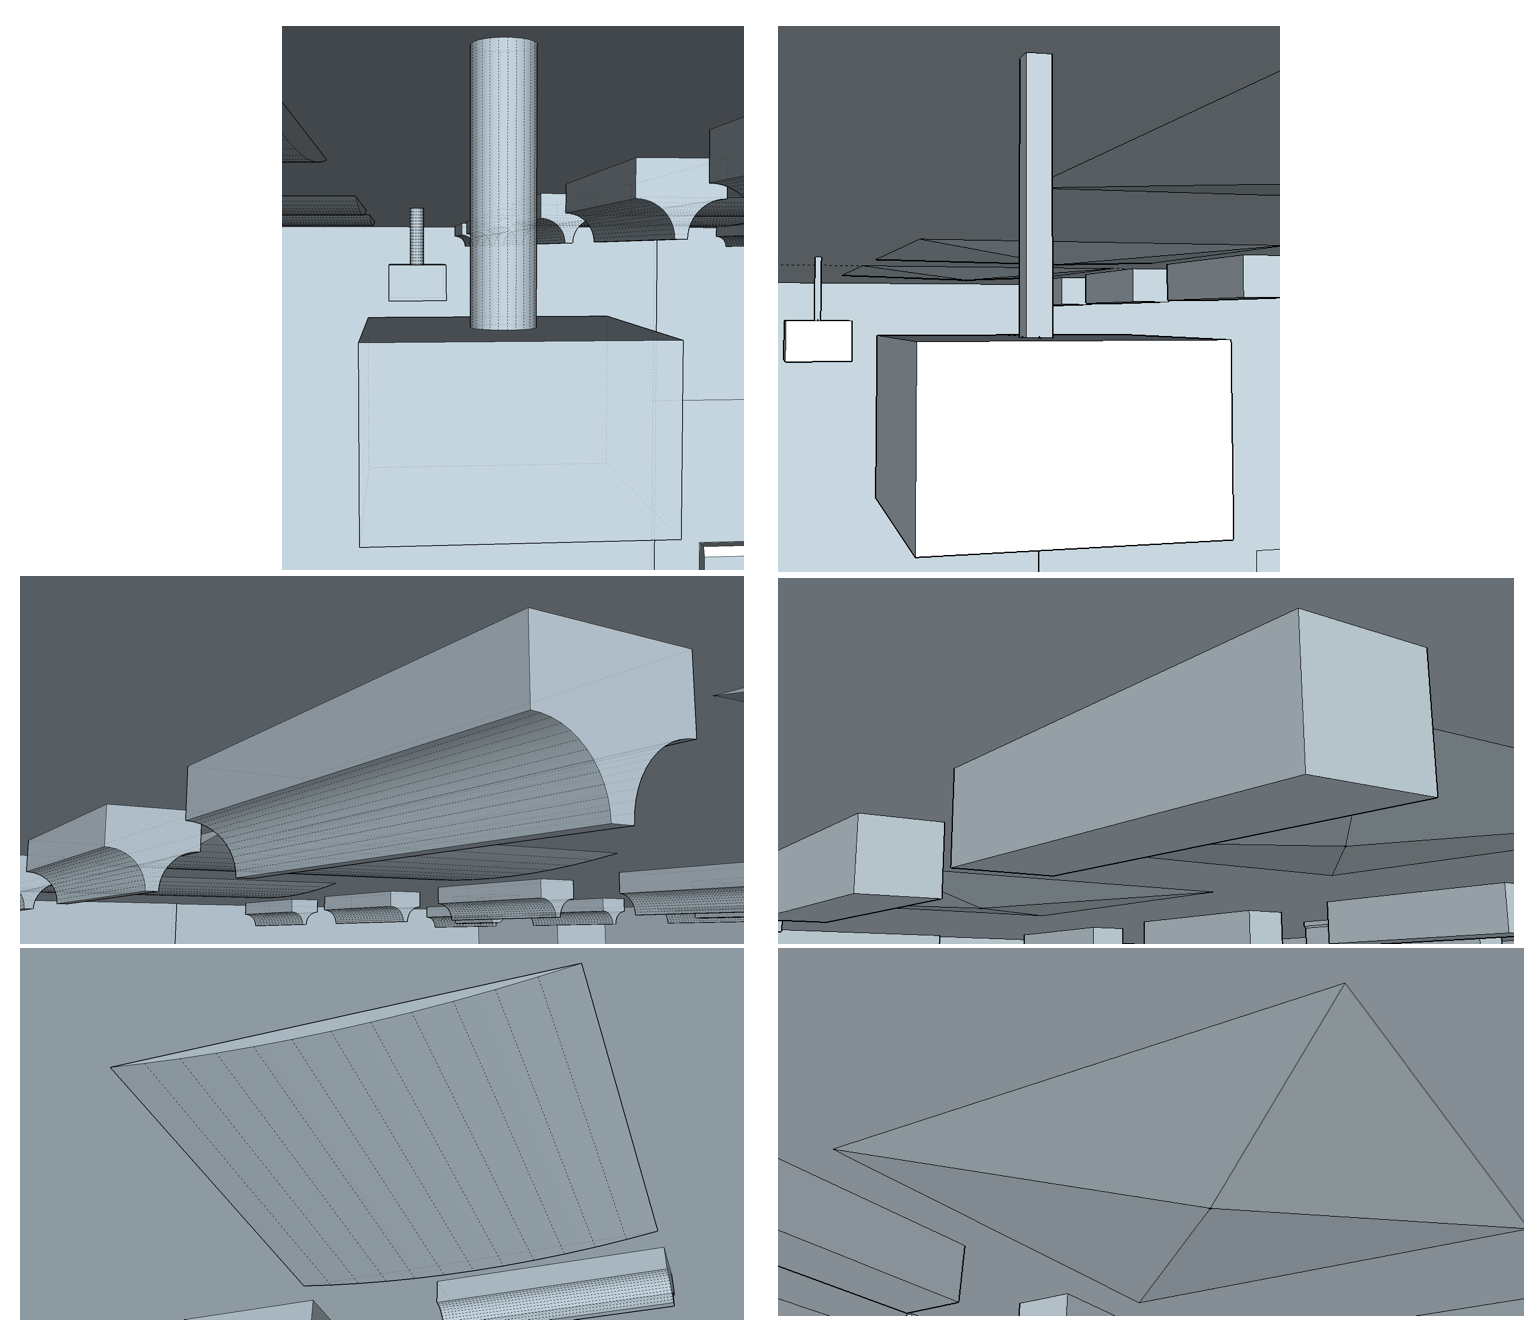
\includegraphics[scale = 0.5]{Sections/Implementation/Modelling/images/SimplevsComplex/all2.png}}
				\caption{Comparison of the original complex models (left) and the their simplified versions (right)}
				\label{compareModels}
			\end{figure}
			


			% \begin{figure}[H]
			% 	\center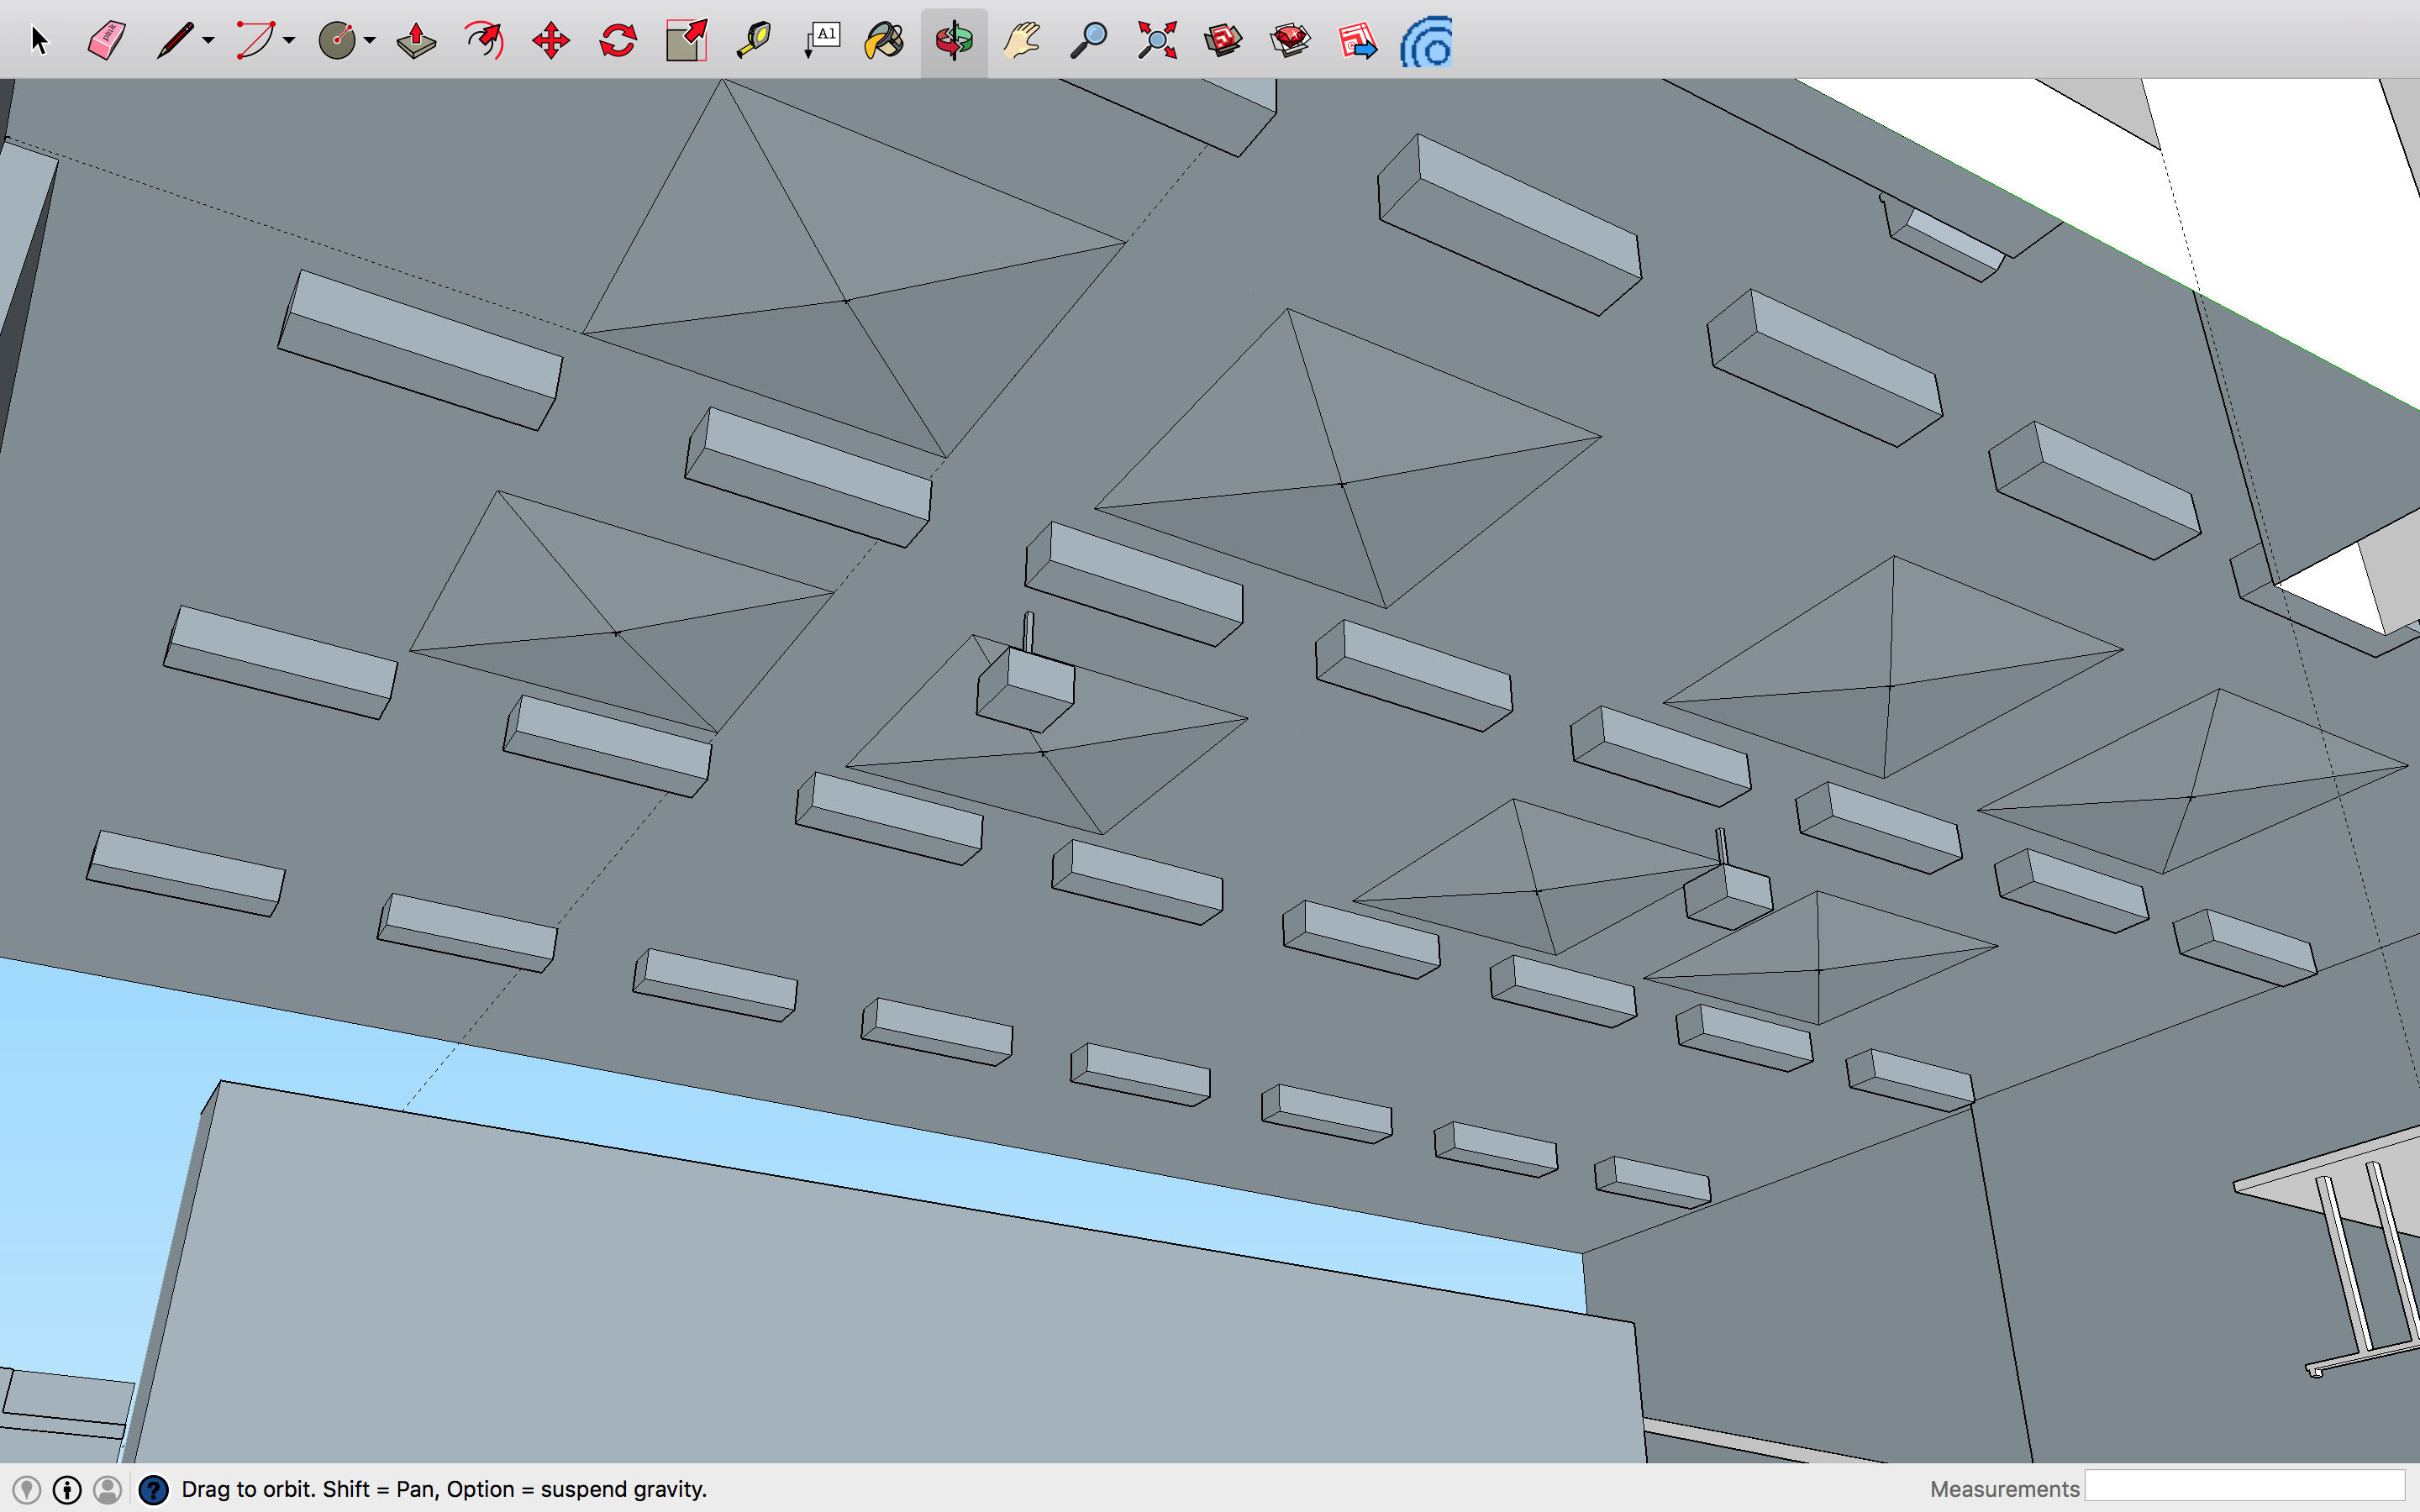
\includegraphics[scale = 0.3]{Sections/Implementation/Modelling/images/realVsSku/roofSku.png}
			% 	\center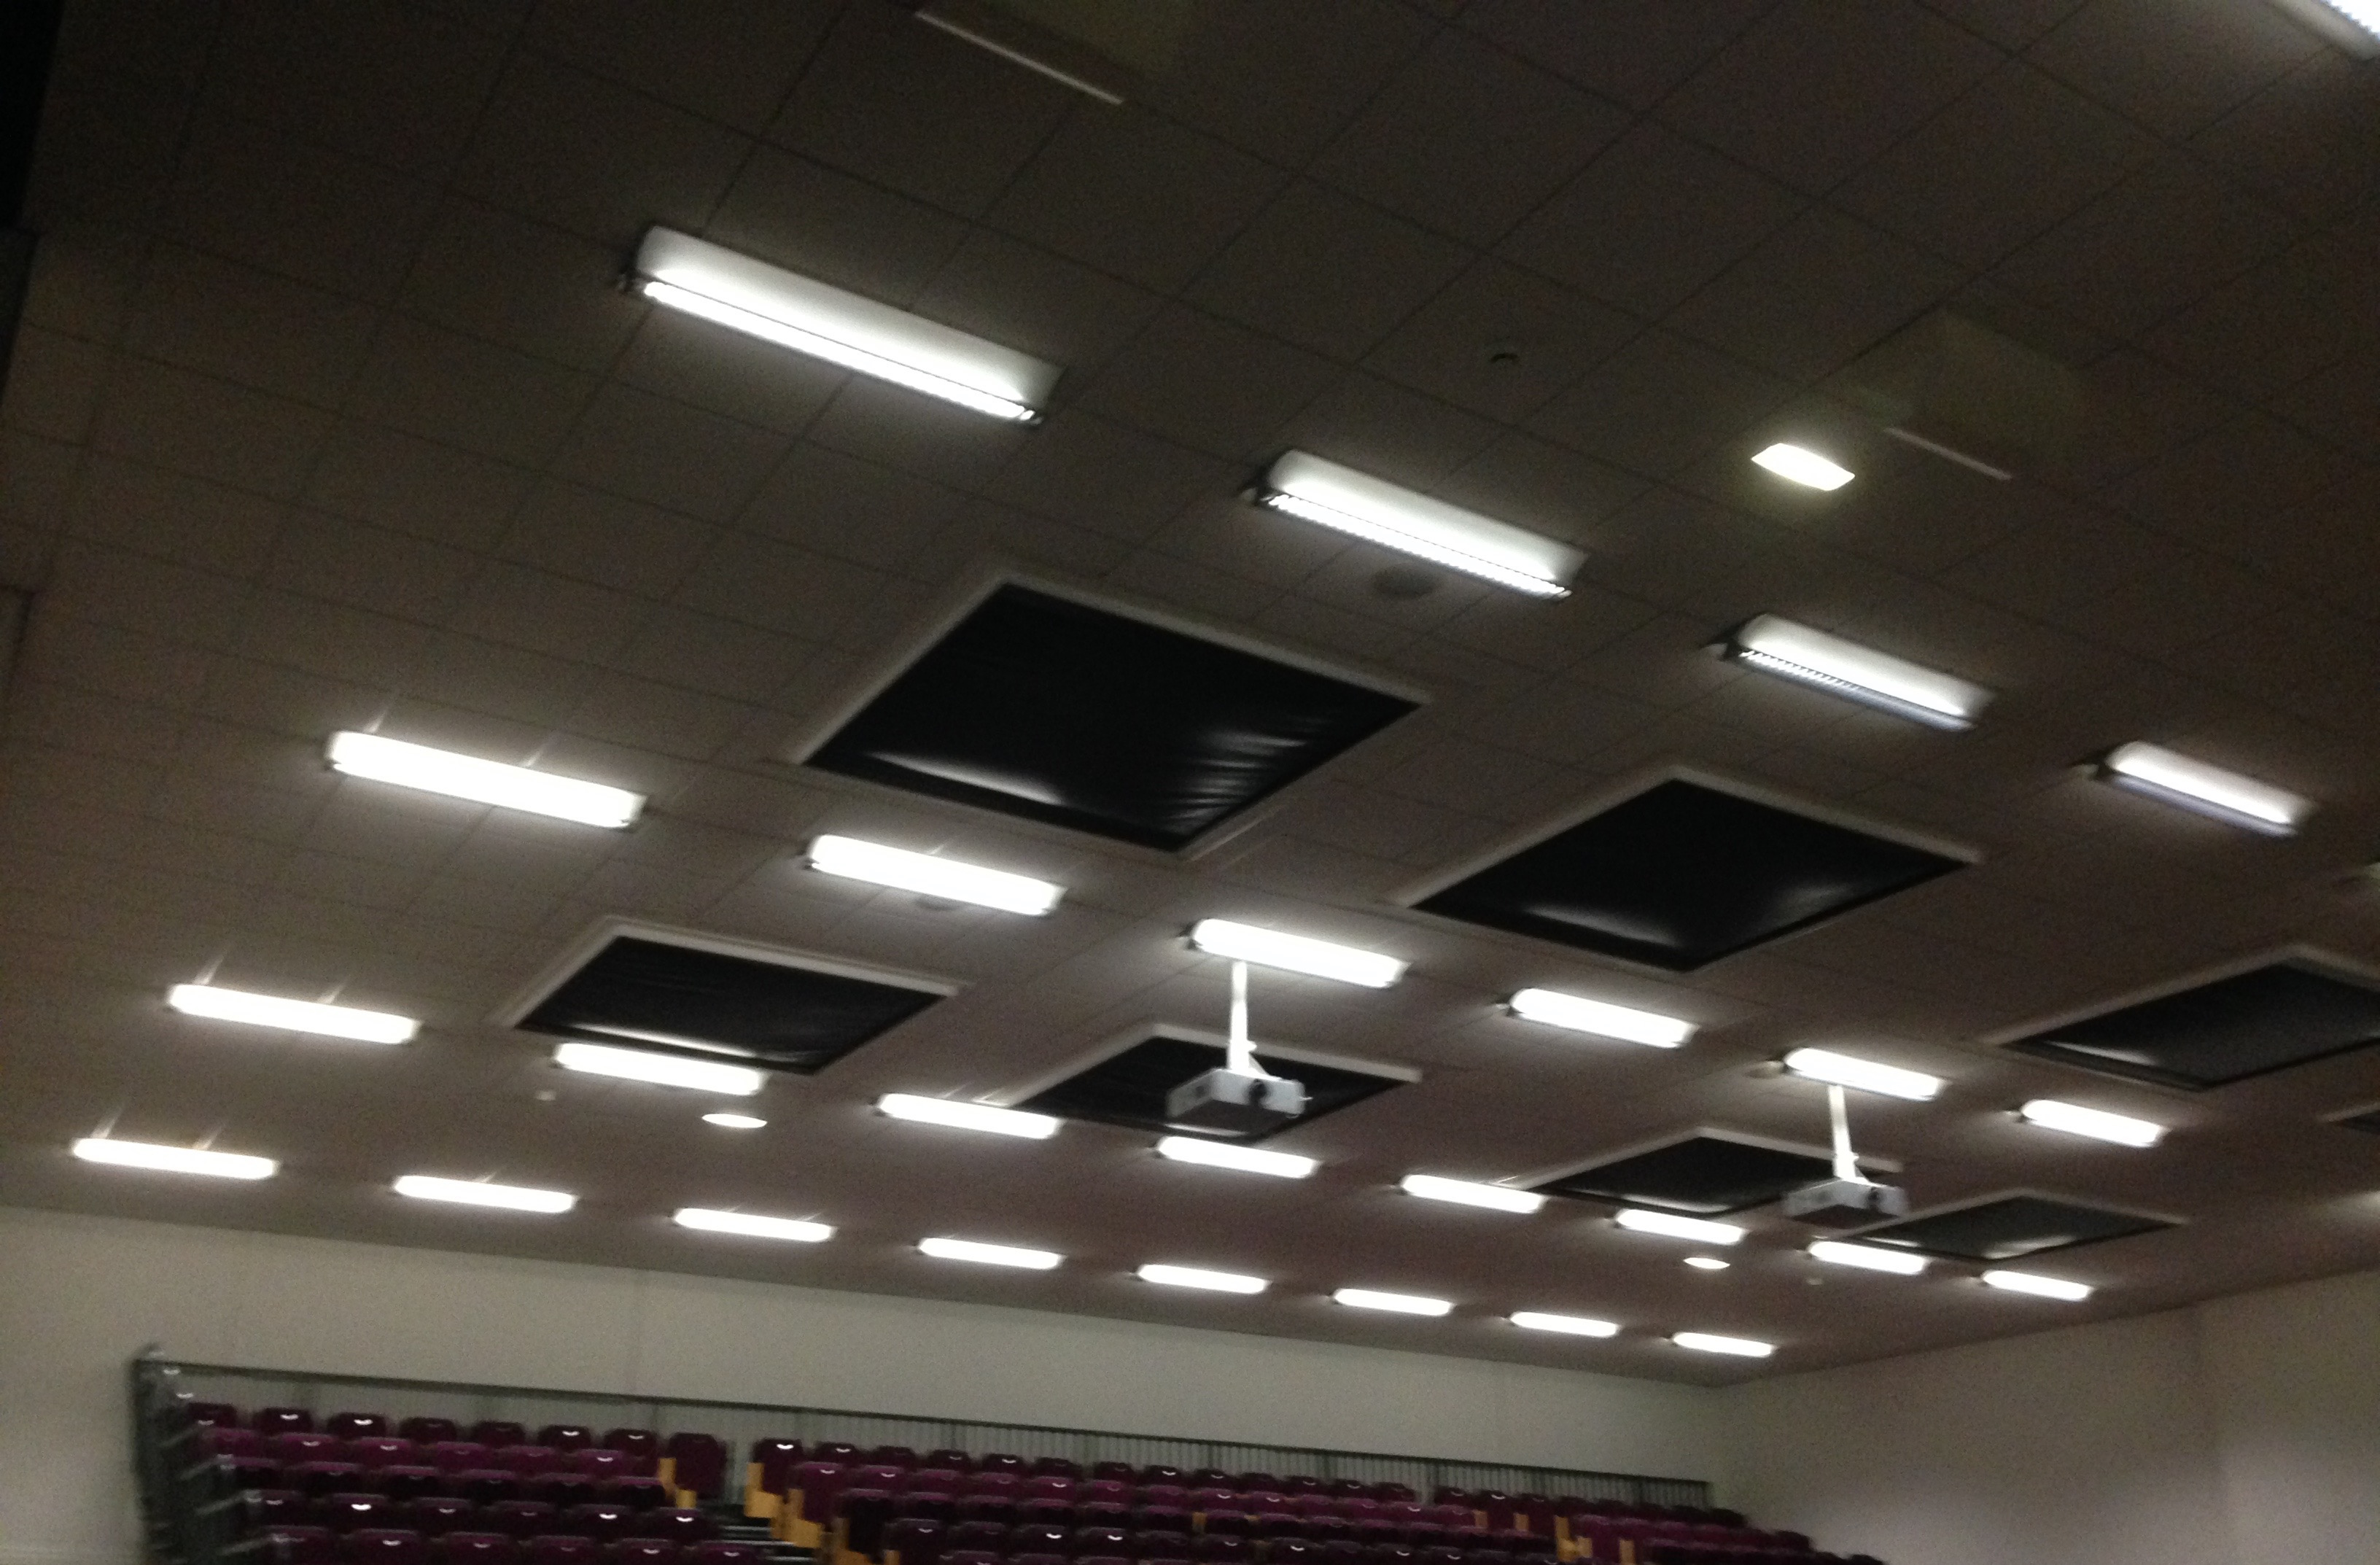
\includegraphics[scale = 0.13]{Sections/Implementation/Modelling/images/HHroof.jpg}
			% 	\caption{Comparison of the final simplified model and a picture of the real Hendrix Hall}
			% 	\label{simpleSurfacesRoom}
			% \end{figure}

\end{document}